\documentclass[12pt, openany]{book}

% ──────────────────────────────────────────────
% Packages
% ──────────────────────────────────────────────
\usepackage[margin=1in]{geometry}
\usepackage{amsmath, amssymb, amsthm}
\usepackage{mathtools}
\usepackage{bm}
\usepackage{float}
\usepackage{graphicx}
\usepackage{tikz}
\usepackage{pgfplots}
\pgfplotsset{compat=1.18}
\usetikzlibrary{arrows.meta, decorations.markings, calc, patterns, positioning}
\usepackage{tcolorbox}
\tcbuselibrary{theorems, breakable, skins}
\usepackage{hyperref}
\usepackage{enumitem}
\usepackage{fancyhdr}
\usepackage{titlesec}
\usepackage{epigraph}
\usepackage{xcolor}
\usepackage{booktabs}

% ──────────────────────────────────────────────
% Colors
% ──────────────────────────────────────────────
\definecolor{chapblue}{RGB}{0, 70, 130}
\definecolor{accentred}{RGB}{180, 40, 40}
\definecolor{softgray}{RGB}{245, 245, 245}
\definecolor{trajgreen}{RGB}{30, 130, 60}
\definecolor{darkgold}{RGB}{160, 120, 20}
\definecolor{purplehaze}{RGB}{100, 40, 140}

% ──────────────────────────────────────────────
% Theorem environments
% ──────────────────────────────────────────────
\newtcbtheorem[number within=chapter]{principle}{Principle}{
  colback=chapblue!5, colframe=chapblue!80,
  fonttitle=\bfseries, separator sign={.~},
  breakable
}{princ}

\newtcbtheorem[number within=chapter]{keyidea}{Key Idea}{
  colback=accentred!5, colframe=accentred!70,
  fonttitle=\bfseries, separator sign={.~},
  breakable
}{idea}

\newtcbtheorem[number within=chapter]{example}{Example}{
  colback=softgray, colframe=black!40,
  fonttitle=\bfseries, separator sign={.~},
  breakable
}{ex}

\newtcbtheorem[number within=chapter]{definition}{Definition}{
  colback=darkgold!5, colframe=darkgold!80,
  fonttitle=\bfseries, separator sign={.~},
  breakable
}{def}

\newtcbtheorem[number within=chapter]{remark}{Remark}{
  colback=purplehaze!5, colframe=purplehaze!60,
  fonttitle=\bfseries, separator sign={.~},
  breakable
}{rem}

\newtcbtheorem[number within=chapter]{warning}{Warning}{
  colback=accentred!5, colframe=accentred!80,
  fonttitle=\bfseries, separator sign={.~},
  breakable
}{warn}

\theoremstyle{plain}
\newtheorem{proposition}{Proposition}[chapter]
\newtheorem{theorem}{Theorem}[chapter]
\newtheorem{lemma}[theorem]{Lemma}
\newtheorem{corollary}[theorem]{Corollary}

% ──────────────────────────────────────────────
% Chapter formatting
% ──────────────────────────────────────────────
\titleformat{\chapter}[display]
  {\normalfont\huge\bfseries\color{chapblue}}
  {\chaptertitlename\ \thechapter}{20pt}{\Huge}
\titlespacing*{\chapter}{0pt}{-20pt}{30pt}

% ──────────────────────────────────────────────
% Header/Footer
% ──────────────────────────────────────────────
\pagestyle{fancy}
\fancyhf{}
\fancyhead[LE,RO]{\thepage}
\fancyhead[RE]{\textit{Control Is Motion}}
\fancyhead[LO]{\textit{\nouppercase{\leftmark}}}
\renewcommand{\headrulewidth}{0.4pt}
\setlength{\headheight}{14.5pt}

% ──────────────────────────────────────────────
% Custom commands
% ──────────────────────────────────────────────
\newcommand{\state}{\bm{x}}
\newcommand{\control}{\bm{u}}
\newcommand{\traj}{\bm{\gamma}}
\newcommand{\manifold}{\mathcal{M}}
\newcommand{\configspace}{\mathcal{Q}}
\newcommand{\statespace}{\mathcal{X}}
\newcommand{\controlspace}{\mathcal{U}}
\newcommand{\Reals}{\mathbb{R}}
\newcommand{\dd}{\mathrm{d}}
\newcommand{\dt}{\,\dd t}
\newcommand{\norm}[1]{\left\lVert #1 \right\rVert}
\newcommand{\inner}[2]{\left\langle #1,\, #2 \right\rangle}

% ──────────────────────────────────────────────
\begin{document}

\setcounter{chapter}{9}

\chapter{Learning to Move}
\label{ch:learning_to_move}
\begingroup
\raggedbottom

\section{What Repetition Can Teach}

A repeated swing provides information: where contact occurred, how the club arrived, and how those outcomes changed after an adjustment. Learning can improve the next command without revealing a unique model of the golfer. It can also overfit a familiar condition, chase measurement noise, or destabilize an otherwise adequate controller. The useful question is which information an update uses and what property that update can actually establish.

This chapter separates three engineering tasks. Iterative learning control adjusts commands between repetitions of a specified task. Policy search chooses parameters of a feedback strategy using a performance objective. System identification estimates a model from observations. These tasks can support one another, but improved tracking, an identified model, and a verified region of successful operation are different results.

For golf, the distinction connects the preceding chapters. A feedforward update changes the forces that exploit inertial coupling. Within-swing feedback changes sensitivity and actuation demands. A phase representation changes how trials are aligned. The impact event determines which deviations matter. A useful learning experiment must preserve these relationships instead of reducing every miss to an arbitrary adjustment of one joint.

\section{Learning Across Trials and Feedback Within a Trial}

Let $j$ index repeated trials over a fixed sampled horizon. Stack the feedforward inputs into $u_j\in\mathbb R^m$ and the measured task outputs into $y_j\in\mathbb R^p$. A local linear lifted model is
\begin{equation}
y_j=G u_j+d,\qquad e_j=r-y_j .
\end{equation}
Here $r$ is the desired output, $d$ is a repeatable offset, and $G$ maps an entire input sequence to an entire output sequence. For a dynamic plant, an earlier command generally affects later measurements. A diagonal, instantaneous learning gain is therefore a special choice, not a representation of all learning laws.

If a fixed feedback controller operates during each trial, $G$ must describe the resulting closed-loop map from feedforward input to output. Define feedback signs using the declared error convention. An offline update can use errors from later in the previous trial without violating causality during the next trial. It cannot use an unmeasured future error from the current swing.

Repeatability concerns the prepared initial state, reference, horizon, contact sequence, measurement alignment, and relevant dynamics. It does not require a perfect model. Changes in fatigue, equipment, ground contact, or sensory delay can nevertheless change the map that an update was designed to improve. Repetitions with different random disturbances must not be silently treated as identical deterministic experiments.

\section{Deriving a Convergence Condition}

Consider the trial update
\begin{equation}
u_{j+1}=Q(u_j+L e_j),
\end{equation}
where $L\in\mathbb R^{m\times p}$ is a learning operator and $Q\in\mathbb R^{m\times m}$ is an optional filter. With $Q=I$ and the same $G,d,r$ on each trial, substitution gives
\begin{equation}
e_{j+1}=(I_p-GL)e_j .
\end{equation}
For this finite-dimensional, fixed linear recursion, spectral radius $\rho(I_p-GL)<1$ implies asymptotic decay of every output error. A chosen induced norm satisfying $\|I_p-GL\|<1$ additionally establishes monotone contraction in that norm. The spectral-radius condition alone does not promise that every intermediate trial improves.

For example, the matrix
\begin{equation}
H=\begin{pmatrix}0.5&4\\0&0.5\end{pmatrix}
\end{equation}
has both eigenvalues equal to $0.5$. Starting from $e_0=(0,1)^\top$ gives $e_1=(4,0.5)^\top$, whose Euclidean norm exceeds four, before eventual decay. Trial-to-trial transients matter when inputs or states have limits. An asymptotic theorem cannot excuse a damaging intermediate trial.

In the scalar plant $G=2$, choosing $L=0.25$ gives $e_{j+1}=0.5e_j$. Choosing $L=1.2$ instead gives $e_{j+1}=-1.4e_j$, which diverges. A larger correction is not necessarily faster learning. Both conclusions follow directly from the actual input-output gain and the sign of the error.

If $G$ lacks full row rank, then $GL$ cannot have full row rank and $I_p-GL$ has eigenvalue one. Arbitrary output references are not all attainable. One can instead analyze an attainable subspace, the component of error that learning can reduce, or a constrained least-squares objective. Input directions in the null space of $G$ are invisible to these outputs; output convergence alone does not guarantee convergence or boundedness of all internal states and commands.

For general $Q$, the command recursion is
\begin{equation}
u_{j+1}=Q(I_m-LG)u_j+QL(r-d).
\end{equation}
If its transition matrix has spectral radius below one, it has a unique attracting fixed point. That point need not give zero error. With $G=2$, $L=0.25$, $Q=0.8$, and $d=0$, the recursion is $u_{j+1}=0.4u_j+0.2r$. It converges to $u_\infty=r/3$, so $y_\infty=2r/3$ and $e_\infty=r/3$. Filtering can improve robustness while introducing bias; it does not remove unwanted information without consequences.

\section{Noise Places a Floor Under Repeated Corrections}

Suppose $G=1$, $d=0$, $Q=1$, and the measured output is $y_j=u_j+\eta_j$, with independent zero-mean measurement noise of variance $R$. For learning gain $0<\ell<2$, the deviation $v_j=u_j-r$ satisfies
\begin{equation}
v_{j+1}=(1-\ell)v_j-\ell\eta_j,\qquad
S_{j+1}=(1-\ell)^2S_j+\ell^2R .
\end{equation}
The stationary command variance is
\begin{equation}
S_\infty=\frac{\ell R}{2-\ell} .
\end{equation}
For $0<\ell\leq1$, a smaller gain reduces this noise floor but slows mean convergence. As $\ell$ approaches two from below, the mean recursion remains asymptotically stable while stationary variance becomes arbitrarily large. This is command variation induced by measurement noise; independent physical trial noise would require its own model and contribution to outcome variability.

Filtering or averaging can reduce a specified noise component. It cannot generally remove all non-repeatable noise while perfectly preserving the signal. Correlation, nonstationarity, and trial-dependent dynamics change the calculation. Report both systematic error and dispersion, along with retained trial counts and measurement uncertainty. A single successful shot does not establish convergence or repeatability.

\begin{figure}[H]
\centering
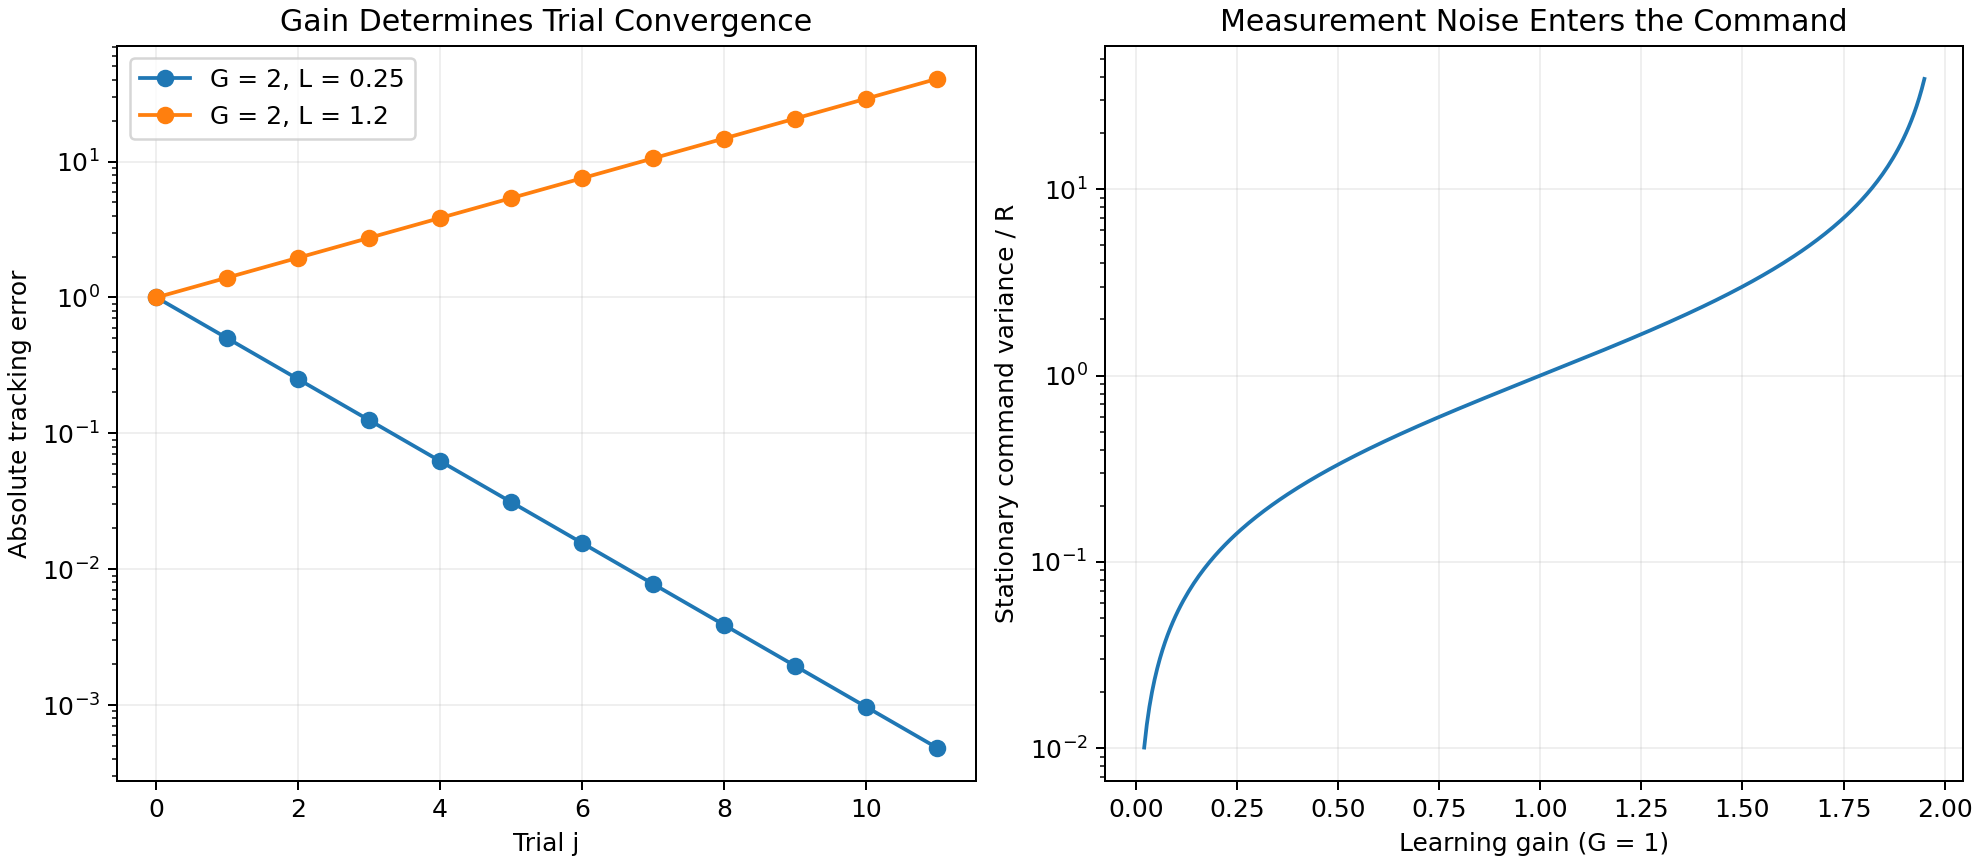
\includegraphics[width=\linewidth]{../The_Geometry_of_Motion/figures/learning_convergence_limits.png}
\caption{Learning Gain Changes Convergence and Noise}
\end{figure}

The figure uses the stated linear recursions. One panel compares convergence and divergence for the scalar plant; the other shows the stationary variance generated by noisy measurements. These are calculated counterexamples, not measured learning curves for golfers.

\section{Tracking Does Not Identify the True Mechanics}

A learning update can compensate a repeatable error on one task without uniquely identifying inertia, stiffness, friction, or neural feedback. In the parameterized model $y=(\theta_1+\theta_2)u$, every pair with the same sum gives the same observations for every input. A command can achieve perfect tracking even though the two parameters remain indistinguishable.

For a linear regression $y_k=\varphi_k^\top\theta+\eta_k$, a finite data set identifies the parameters in the noise-free model only if its regressor matrix has full column rank. Persistent excitation is a related time-dependent richness condition used in identification and adaptation. Its precise form depends on the estimator and model. It is not equivalent to exciting the full control Lie algebra. Controllability concerns possible motions; identifiability concerns distinguishable models from the available observations.

The geometric constraints of earlier chapters still matter: the commands must generate feasible motions under actuation and contact limits. ILC convergence is not convergence to the boundary of a Lie orbit or reachable set. A tracking reference can lie in the interior of a reachable set, and unmodeled dynamics need not be reconstructed for that one reference to improve.

For nonlinear mechanics, a lifted Jacobian can support a local learning calculation. Changing the nominal motion, crossing a contact transition, or encountering saturation can invalidate that linearization. Projecting an updated command into actuator bounds changes the recursion and requires a constrained analysis. Phase-aligning trials also changes the input-output map: derivatives, phase speed, event timing, and interpolation must be treated consistently. Alignment should not erase an impact-speed error that the task actually penalizes.

\section{Policy Search Optimizes Its Declared Objective}

A policy $u=\pi_\theta(\hat x,s)$ may depend on an estimated state and a phase variable. Policy search adjusts $\theta$ using a stated criterion such as expected impact reward minus effort or dispersion penalties. Its observations, actuator limits, contact model, disturbance distribution, and termination rule are part of the problem. Optimizing a scalar reward does not automatically compute or enlarge a certified funnel.

For a differentiable stochastic policy, assume the initial-state distribution and environment transition law do not depend directly on $\theta$. A finite-horizon likelihood-ratio identity then has the form
\begin{equation}
\nabla_\theta J
=\mathbb E\!\left[\sum_{k=0}^{N-1}
\nabla_\theta\log\pi_\theta(u_k\mid h_k)\,R_k\right],
\end{equation}
where $h_k$ is the available history and $R_k$ is the remaining return. The identity requires differentiability, integrability, and interchange of derivative and expectation; policy support and parameter-dependent rewards require appropriate treatment. Estimated gradients have sampling error. Convergence results require further assumptions and generally do not establish a global optimum in a nonlinear policy family.

A finite reward penalty is also different from a hard constraint. With finite $\lambda>0$, consider
\begin{equation}
\max_{u\in\mathbb R}\{u-\lambda\max(0,u-1)^2\},\qquad
u^\star=1+\frac{1}{2\lambda}>1 .
\end{equation}
The quadratic penalty reduces the violation but never enforces the desired upper bound exactly in this example. Enforce actuator bounds and other required constraints explicitly, or establish the relevant constrained or probabilistic guarantee.

A trained policy might use phase information, exploit coupled dynamics, or reduce feedback in a noisy direction. Those are hypotheses to test by inspecting a trained policy and comparing controlled alternatives. They are not universal outcomes of reinforcement learning. A plausible swing animation cannot establish that the policy found a specific biological mechanism or a robust region of attraction.

Population-based and other derivative-free searches can evaluate policy parameters when useful gradients are unavailable. They still optimize the supplied objective using a finite evaluation budget. Contact discontinuities, simulator errors, and reward loopholes do not disappear. A candidate discovered by any search method remains subject to independent dynamics, constraint, and outcome checks.

\section{Valid Entry and Transfer in a Trajectory Library}

Store more than a nominal motion. A useful library entry records its reference, feedback policy, state and phase coordinates, actuator and sensing assumptions, admissible initial set, disturbance/model domain, terminal task, and any verified certificate. A certificate for one equipment configuration or contact mode does not automatically cover another.

Similarity in a task descriptor can retrieve a candidate. Actual reuse requires the current state, or the relevant state-uncertainty set, to satisfy the entry conditions under the applicable assumptions. To concatenate entries, the previous terminal set, including any reset image and timing conditions, must lie inside the next valid initial set. Membership near impact does not establish that the preceding swing remains admissible.

LQR-Trees constructs a tree of locally stabilized trajectories connected toward a goal and associates them with verified regions. It does not establish that arbitrary interpolation of two stored controllers yields a stable controller. Its asymptotic coverage results depend on sampling, planning, stabilization, and verification assumptions; they are not a finite-data guarantee for a learned golf policy.

The interpolation problem appears even in linear systems. Let
\begin{equation}
A_1=\begin{pmatrix}-1&4\\0&-1\end{pmatrix},\qquad
A_2=\begin{pmatrix}-1&0\\4&-1\end{pmatrix}.
\end{equation}
Both continuous-time systems are asymptotically stable, but their equal-weight average has eigenvalues $1$ and $-3$ and is unstable. Similarly, two feasible paths passing on opposite sides of an obstacle can have an average that passes through it. Stability and feasibility are properties to check, not consequences of visual similarity.

There are useful special cases. If a family of closed-loop matrices shares a positive-definite quadratic Lyapunov matrix $P$ with $A_i^\top P+PA_i\prec0$, then convex combinations preserve that inequality. Such a common certificate, together with valid region, input, and contact conditions, can support blending. Separate certificates with different metrics do not supply that conclusion automatically.

A retrieved or blended motion can instead serve as a warm start for optimization. That is an initial guess. After adaptation, verify dynamic feasibility, input and contact bounds, relevant perturbations, the full interval, and the terminal event. Recompute or revalidate a certificate when the controller or its assumptions change. Do not label a successful simulation as a certified funnel.

\section{A Learning Experiment That Can Inform Golf}

First declare the outcome: contact location, face orientation, speed, launch conditions, or a weighted combination with meaningful units. Measure enough of the motion and environment to test the proposed mechanism. Keep the within-swing feedback and across-swing update distinct, and record all attempted trials, including misses and saturation.

Then compare alternatives under matched information and limits. A time-based and phase-based controller should receive comparable observations and actuation authority. An effort penalty and a dispersion penalty should be evaluated against the same contact task. Test sensitivity to initial state, timing, equipment parameters, and measurement delay. Use held-out conditions and random realizations, and distinguish improvement during adaptation from retention and transfer after the update is stopped.

If an adjustment improves contact, determine whether it changed mean bias, variance, timing sensitivity, energy transfer, or several of these together. Those mechanisms can interact: altered coordination changes mechanical sensitivity; altered feedback changes both disturbance rejection and noise amplification; altered speed changes contact-event timing. The engineering model helps formulate discriminating predictions. Evidence that an athlete improved does not by itself identify the athlete's internal objective or learning algorithm.

\begin{samepage}
\section{Primary Reading}

\href{https://www.diag.uniroma1.it/~deluca/rob2_en/A_survey_of_iterative_learning_control_CSMag_2006.pdf}{Bristow, Tharayil, and Alleyne (2006)} surveys lifted ILC, convergence, filtering, and robustness.
\href{https://proceedings.neurips.cc/paper/1999/file/464d828b85b0bed98e80ade0a5c43b0f-Paper.pdf}{Sutton, McAllester, Singh, and Mansour (1999)} develops policy-gradient results with function approximation.
\href{https://groups.csail.mit.edu/robotics-center/public_papers/Tedrake10.pdf}{Tedrake, Manchester, Tobenkin, and Roberts (2010)} describes LQR-Trees and the assumptions behind its verification and coverage results.
The examples and golf-testing framework here are independently derived interpretations, not reported results from those papers.

\section{Worked Checks and Exercises}

\begin{enumerate}[itemsep=0.25em,parsep=0pt]
\item Derive the lifted error recursion with the stated error sign and dimensions.
\item Verify transient growth for $H$ and convergence or divergence for both scalar learning gains.
\item Calculate the biased fixed point introduced by the stated filter.
\item Derive the stationary command variance under independent measurement noise.
\item Explain why perfect tracking cannot separate the two indistinguishable parameters.
\item Verify the finite-penalty constraint violation and the unstable average of stable systems.
\item State sufficient common-certificate conditions for a proposed controller blend.
\item Design a comparison that distinguishes better impact outcomes from identification of a biological learning mechanism.
\end{enumerate}
\end{samepage}
\clearpage
\endgroup

\end{document}
